\documentclass{article}
\usepackage[utf8]{inputenc}
\usepackage{hyperref}
\usepackage{graphicx}
\usepackage{subcaption}
\usepackage{cite}
\usepackage{float}
\usepackage{etoc}
\usepackage{blindtext}
\usepackage{amsmath}
\usepackage{amssymb}


%quote
\usepackage{epigraph}
\setlength\epigraphwidth{0.505\textwidth}
\setlength\epigraphrule{0pt}

% margins
\usepackage[a4paper, total={6in, 10in}]{geometry}

% spacing
\setlength{\parindent}{0em}
\setlength{\parskip}{1em}

% fonts (the same as NIPS 2016)
\renewcommand{\rmdefault}{ptm}
\renewcommand{\sfdefault}{phv}

\title{Hry v normální formě\vspace{-1em}}
\author{Tomáš Vlk (vlktoma5@fit.cvut.cz)}
\date{\today}

\begin{document}

\maketitle

\section*{Úvod}

Hry v normální formě jsou tvořeny maticí. Konečná hra v normální formě pro $n$ hráčů je trojice $(N, A, u)$, kde:

\begin{enumerate}
\item $N = \{ N_1, \dots, N_n\}$ je konečná množina hráčů
\item $A = A_1 \times \dots \times A_n$, kde $A_i$ je množina akcí, které má k dispozici hráč $N_i$. $\boldsymbol{a} \in A$ je takzvaný akční profil, vyjadřující jednu konkrétní volbu akcí provedenou nezávisle všemi hráči ve hře.
\item $u =  (u_1, \dots, u_n)$ je posloupnost utilitních akci pro jednotlivé hráče. $u_i: A \rightarrow \mathbb{R}$ a $u_i(\boldsymbol{a})$ vyjadřuje utilitu hráče $N_i$ z akčního profilu $\boldsymbol{a} \in A$.
\end{enumerate}

Utilitní funkce hráče udává výhodnot/nevýhodnost danné situace pro svého hráče.

\section*{Kanonické hry v normální formě}

Ve hrách v normální jsou hráči rovnocení a nezáleží na tom který z nich vyhraje. Hlavním využitím je hledání optimálních akčních profilů.

\subsection*{Common-payoff hra}

Pokud uvažujeme hru v normální formě $G = (N, A, u)$, pak je common-payoff hrou právě v případě, že $\forall \boldsymbol{a} \in A: u_1(\boldsymbol{a}) = u_2(\boldsymbol{a}) = \dots = u_n(\boldsymbol{a})$. Příkladem common-payoff hry může například být "Po které straně silnice jezdit", viz. Obrázek \ref{fig:roadSide}.

\begin{figure}[h]
\begin{center}
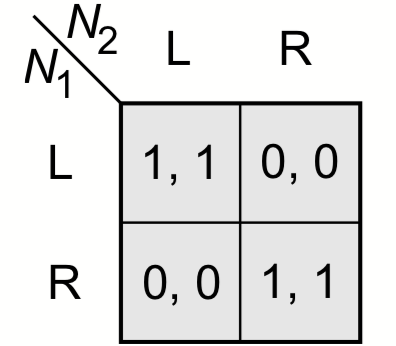
\includegraphics[scale=0.8]{LeftOrRight}
\caption{"Po které staně silnice jezdit"}
\label{fig:roadSide}
\end{center}
\end{figure}

\subsection*{Constant-sum hra}

Pokud uvažujeme hru v normální formě $G = (N, A, u)$, pak je constant-sum hrou přávě tehdy, když $\exists c \in \mathbb{R}: \forall \boldsymbol{a} \in A: \sum_{i = 1}^{n} u_i(\boldsymbol{a}) = c$. Speciální případ, kdy $c = 0$ se nazývá zero-sum hrou. Příkladem takovéto hry je například kámen-nůžky-papír, viz. Obrázek \ref{fig:knp}.

\begin{figure}[h]
\begin{center}
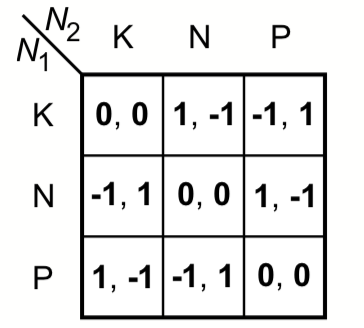
\includegraphics[scale=0.8]{KNP}
\caption{Kámen-Nůžky-Papír}
\label{fig:knp}
\end{center}
\end{figure}

\section*{Akční profily}

Mezi akční profily patří například:

\begin{itemize}
\item \textbf{Paretovo optimum} - Žádnou změnou akčního profilu již hráč nemůže zvýšit svou utilitu, aniž by se snížila utilita jiných hráčů.

\item \textbf{Nashovo equlibrium} - Žádný hráč nemůže žádnou akcí zvýšit svou utilitu, akční profil je tedy stabilní. Žádný hráč není motivován změnit své rozhodnutí.
\end{itemize}

\subsection*{Paretovo optimum}

Mějme hru v normální formě $(N, A, u)$, kde $u=(u_1, u_2, \dots, u_n)$, pak akční profil $\boldsymbol{a'} = (a'_{N_1}, a'_{N_2}, \dots, a'_{N_n}) \in A$ je \textbf{paretovsky dominantní} nad akčním profilem $\boldsymbol{a} = (a_{N_1}, \dots, a_{N_n}) \in A$, pokud platí následující podmínky:

\begin{enumerate}
\item $\forall i \in \{1, \dots, n\}: u_i(\boldsymbol{a'}) \geq u_i(\boldsymbol{a})$

\item $\exists i \in \{ 1, \dots, n\}: u_i(\boldsymbol{a'})  > u_i(\boldsymbol{a})$
\end{enumerate}

Pokud tedy máme hru v normální formě $(N, A, u)$, pak je akční profil $\boldsymbol{a*} \in A$ je paretovsky optimální, jestliže neexistuje akční profil $\boldsymbol{a'} \in A$, který jej paretovsky dominuje. Ukázka v Obrázku \ref{fig:paret}.

\begin{figure}[h]
\begin{center}
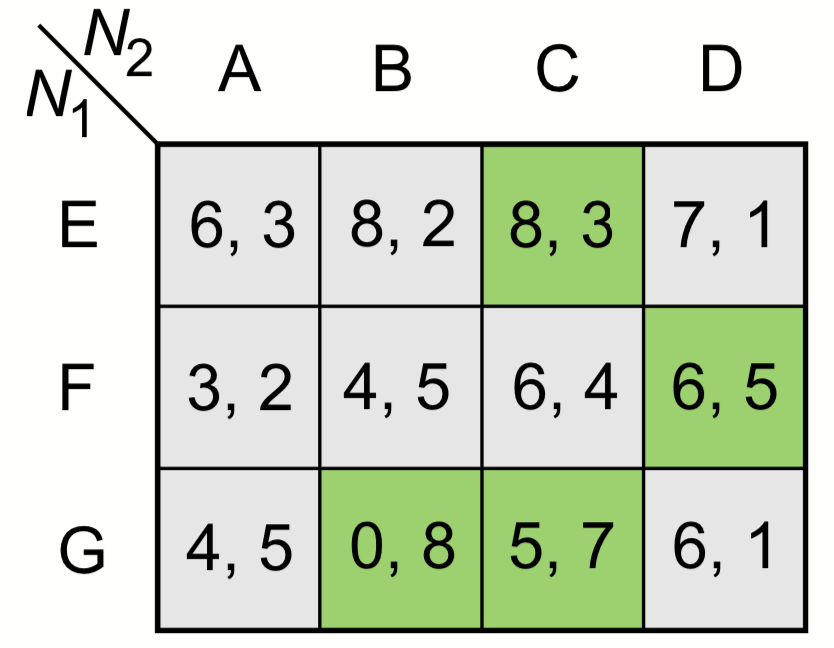
\includegraphics[scale=0.6]{Paret}
\caption{Paretovo optimum}
\label{fig:paret}
\end{center}
\end{figure}

\subsection*{Nashovo equlibrium}

Hry v normální formě mají omezenou pozorovatelnost, jelikož hráči volí své akce nezávisle na ostatních. Pokud by hráč veděl, jaké akce zvolili ostatní hráči, mohl by snadno zvolit optimální akci. Tato volba optimální akce se nazývá \textbf{Best Response}.\par

Formálně pokud máme hru v normální formě $(N, A, u)$, akční profil $\boldsymbol{a}=(a_{N_1}, a_{N_2}, \dots, a_{N_n})$, hráče $N_i \in N$ a jeho utilitní funkci $u_i$. Potom je $\boldsymbol{a}_{-i}=(a_{N_1}, \dots,a_{N_{i-1}}, a_{N_{i+1}}, \dots, a_{N_n})$ je redukovaný akční profil všech hráčů krom hráče $N_i$.\par 

Best response na $\boldsymbol{a}_{-i}$ pak je množina $BR(\boldsymbol{a_{-i}}) = \arg \max\limits_{\hat{a}_{N_i} \in A_i} u_i((a_{N_i}, \dots, a_{N_{i-1}}, \hat{a}_{N_i}, a_{N_{i+1}}, \dots, a_{N_n}))$.\par 

Mějme hru v normální formě $(N, A, u)$ a akčním profilu $\boldsymbol{a} = (a_{N_1}, a_{N_2}, \dots, a_{N_n})$. Pak akční profil $\boldsymbol{a}$ je \textbf{Nashovým equalibriem}, pokud $$\forall i \in \{1, \dots, n\}: a_{N_i} \in BR(\boldsymbol{a}_{-i})$$

Nashovo equalibrium je tedy takový akční profil, kde akce každého hráče představuje best response na akce všech ostatních hráčů. Ukázka v Obrázku \ref{fig:nash}.

\begin{figure}[h]
\begin{center}
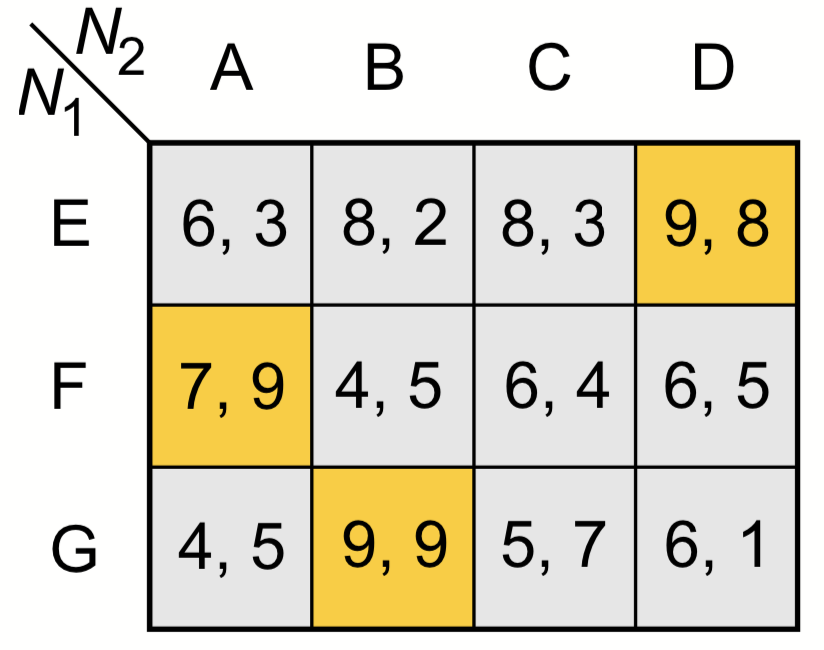
\includegraphics[scale=0.6]{Nash}
\caption{Nashovo equlibrium}
\label{fig:nash}
\end{center}
\end{figure}

\end{document}
